\chapter{Class Lfsr}

\index{LFSR}
\Lfsr\ is an object type allowing to simulate and analyze any type of Linear Feedback Shift Register. Simulations are performed using \texttt{bitarray} objects, where \texttt{bitarray\_object[N]} holds value of Flip-Flop having index \textit{N}. \Lfsr\ objects are always simulated assuming, that data is shifted from higher to lower indexed flip-flop (from FF[1] to FF[0], from FF[2] to FF[1] and so on).

\section{Lfsr types}

\subsection{Fibonacci}

\index{LFSR!Fibonacci}
\index{Fibonacci LFSR}

Look at the Figure \ref{lfsr:fibonacci}. It shows an example of Fibonacci LFSR implementing the polynomial of $x^8+x^6+x^5+x^2+1$. There are couple of ways to create such \Lfsr\ object:

\begin{lstlisting}[language=Python]
	# using existing Polynomial object:
	p1 = Polynomial([8,6,5,2,0])
	lfsr1 = Lfsr(p1, FIBONACCI)
	# using Polynomial created in place:
	lfsr1 = Lfsr(Polynomial([8,6,5,2,0]), FIBONACCI)
	# using coefficients list:
	lfsr1 = Lfsr([8,6,5,2,0], FIBONACCI)
\end{lstlisting}

\begin{figure}[h]
	\centering
	\scalebox{.75}{\newcommand{\drawff}[2]{		
	\fill[black!5!white] 		($#1-(0.5, 0.5)$)	rectangle	($#1+(0.5, 0.5)$);
	\draw[thick] 		($#1-(0.5, 0.5)$)	rectangle	($#1+(0.5, 0.5)$);
	\node[] at ($#1+(0.0, 0.0)$) {\large#2};
}
\newcommand{\drawfibonacciconnector}[2]{
	\draw[-latex] ($#1+(0.0, 0.0)$) -- ($#1+(0.0, 2.0)-(0.0,0.25)$);
	\fill[black]  ($#1+(0.0, 0.0)$) circle (0.07);
	\fill[black!5!white]  ($#1+(0.0, 2.0)$) circle (0.25);
	\draw[thick]  ($#1+(0.0, 2.0)$) circle (0.25);
	\draw[thick]  ($#1+(0.0, 2.0)-(0.25,0.0)$) -- ($#1+(0.0, 2.0)+(0.25,0.0)$);
	\draw[thick]  ($#1+(0.0, 2.0)-(0.0,0.25)$) -- ($#1+(0.0, 2.0)+(0.0,0.25)$);
	\draw[latex-] ($#1+(0.0, 2.0)+(0.25,0.0)$) -- ($#1+(0.0, 2.0)+(0.5,0.0)$);
	\node[anchor=west] at ($#1+(0.0, 1.2)$) {\Large#2};
}
\begin{tikzpicture}
	\draw (-1,0) rectangle (15,2);
	\drawff {(0,0)} {7}
	\drawff {(2,0)} {6}
	\drawfibonacciconnector {(3,0)} {$x^6$}
	\drawff {(4,0)} {5}
	\drawfibonacciconnector {(5,0)} {$x^5$}
	\drawff {(6,0)} {4}
	\drawff {(8,0)} {3}
	\drawff {(10,0)} {2}
	\drawfibonacciconnector {(11,0)} {$x^2$}
	\drawff {(12,0)} {1}
	\drawff {(14,0)} {0}
	\draw[-latex] (-1.0,0.0) -- (-0.5,0.0);
\end{tikzpicture}}
	\caption{Fibonacci LFSR implementing polynomial $x^8+x^6+x^5+x^2+1$.}
	\label{lfsr:fibonacci}
\end{figure}

\subsection{Galois}

\index{LFSR!Galois}
\index{Galois LFSR}

Figure \ref{lfsr:fibonacci} shows an example of Galois LFSR implementing the polynomial of $x^8+x^6+x^5+x^2+1$. There are couple of ways to create such \Lfsr\ object:

\begin{lstlisting}[language=Python]
	# using existing Polynomial object:
	p1 = Polynomial([8,6,5,2,0])
	lfsr1 = Lfsr(p1, GALOIS)
	# using Polynomial created in place:
	lfsr1 = Lfsr(Polynomial([8,6,5,2,0]), GALOIS)
	# using coefficients list:
	lfsr1 = Lfsr([8,6,5,2,0], GALOIS)
\end{lstlisting}

\begin{figure}[h]
	\centering
	\scalebox{.75}{\newcommand{\drawff}[2]{		
	\fill[black!5!white] 		($#1-(0.5, 0.5)$)	rectangle	($#1+(0.5, 0.5)$);
	\draw[thick] 		($#1-(0.5, 0.5)$)	rectangle	($#1+(0.5, 0.5)$);
	\node[] at ($#1+(0.0, 0.0)$) {\large#2};
}
\newcommand{\drawgaloisconnector}[2]{
	\draw[latex-] ($#1+(0.0, 0.25)$) -- ($#1+(0.0, 2.0)-(0.0,0.0)$);
	\fill[black]  ($#1+(0.0, 2.0)$) circle (0.07);
	\fill[black!5!white]  ($#1+(0.0, 0.0)$) circle (0.20);
	\draw[thick]  ($#1+(0.0, 0.0)$) circle (0.2);
	\draw[thick]  ($#1+(0.0, 0.0)-(0.2,0.0)$) -- ($#1+(0.0, 0.0)+(0.2,0.0)$);
	\draw[thick]  ($#1+(0.0, 0.0)-(0.0,0.2)$) -- ($#1+(0.0, 0.0)+(0.0,0.2)$);
	\draw[latex-] ($#1+(0.0, 0.0)-(0.5,0.0)$) -- ($#1+(0.0, 0.0)-(0.2,0.0)$);
	\node[anchor=west] at ($#1+(0.0, 1.2)$) {\Large#2};
}
\begin{tikzpicture}
	\draw (-1,0) rectangle (15,2);
	\drawff {(0,0)} {7}
	\drawff {(2,0)} {6}
	\drawgaloisconnector {(3,0)} {$x^6$}
	\drawff {(4,0)} {5}
	\drawgaloisconnector {(5,0)} {$x^5$}
	\drawff {(6,0)} {4}
	\drawff {(8,0)} {3}
	\drawff {(10,0)} {2}
	\drawgaloisconnector {(11,0)} {$x^2$}
	\drawff {(12,0)} {1}
	\drawff {(14,0)} {0}
	\draw[-latex] (-1.0,0.0) -- (-0.5,0.0);
\end{tikzpicture}}
	\caption{Galois LFSR implementing polynomial $x^8+x^6+x^5+x^2+1$.}
	\label{lfsr:galois}
\end{figure}

\subsection{Ring Generator}

\index{LFSR!Ring Generator}
\index{Ring Generator}

Ring generator is a structure discussed in \cite{lfsr:fastsim}. Example of a Ring Generator is shown in the Figure \ref{lfsr:ring} implementing the polynomial $x^8+x^6+x^5+x^2+1$. Ways to create such object are:

\begin{lstlisting}[language=Python]
	# using existing Polynomial object:
	p1 = Polynomial([8,6,5,2,0])
	lfsr1 = Lfsr(p1, RING_GENERATOR)
	# using Polynomial created in place:
	lfsr1 = Lfsr(Polynomial([8,6,5,2,0]), RING_GENERATOR)
	# using coefficients list:
	lfsr1 = Lfsr([8,6,5,2,0], RING_GENERATOR)
\end{lstlisting}

\begin{figure}[h]
	\centering
	\scalebox{.75}{\newcommand{\drawff}[2]{		
	\fill[black!5!white] 		($#1-(0.5, 0.5)$)	rectangle	($#1+(0.5, 0.5)$);
	\draw[thick] 		($#1-(0.5, 0.5)$)	rectangle	($#1+(0.5, 0.5)$);
	\node[] at ($#1+(0.0, 0.0)$) {\large#2};
}
\newcommand{\drawring}[2]{
	\coordinate (A) at ($#1-(1.0,0.0)$);
	\coordinate (A2) at ($(A)+(0.5,0.0)$);
	\coordinate (B) at ($#2+(1.0,0.0)$);
	\coordinate (B2) at ($(B)-(0.5,0.0)$);
	\draw (A) rectangle (B);
	\draw[-latex] (A) -- (A2);
	\draw[-latex] (B) -- (B2);
}
\newcommand{\drawringconnectorup}[3]{
	\coordinate (A) at ($#1+(0.0,1.0)$);
	\coordinate (B) at ($#2-(0.0,1)$);
	\coordinate (C) at ($0.3*(B)+0.7*(A)+(0.0,0.2)$);
	\draw[-latex] #1 -- (A) -- (B) -- ($#2-(0.0,0.2)$);
	\fill[black]  ($#1+(0.0, 0.0)$) circle (0.07);
	\fill[black!5!white]  ($#2+(0.0, 0.0)$) circle (0.20);
	\draw[thick]  ($#2+(0.0, 0.0)$) circle (0.2);
	\draw[thick]  ($#2+(0.0, 0.0)-(0.2,0.0)$) -- ($#2+(0.0, 0.0)+(0.2,0.0)$);
	\draw[thick]  ($#2+(0.0, 0.0)-(0.0,0.2)$) -- ($#2+(0.0, 0.0)+(0.0,0.2)$);
	\node[anchor=west] at (C) {\Large#3};
}
\newcommand{\drawringconnectordown}[3]{
\coordinate (A) at ($#1-(0.0,1.0)$);
\coordinate (B) at ($#2+(0.0,1)$);
\coordinate (C) at ($0.3*(A)+0.7*(B)+(0.0,0.2)$);
\draw[-latex] #1 -- (A) -- (B) -- ($#2+(0.0,0.2)$);
\fill[black]  ($#1+(0.0, 0.0)$) circle (0.07);
\fill[black!5!white]  ($#2+(0.0, 0.0)$) circle (0.20);
\draw[thick]  ($#2+(0.0, 0.0)$) circle (0.2);
\draw[thick]  ($#2+(0.0, 0.0)-(0.2,0.0)$) -- ($#2+(0.0, 0.0)+(0.2,0.0)$);
\draw[thick]  ($#2+(0.0, 0.0)-(0.0,0.2)$) -- ($#2+(0.0, 0.0)+(0.0,0.2)$);
\node[anchor=west] at (C) {\Large#3};
}
\begin{tikzpicture}
	\drawring {(0,0)} {(6,3)};
	
	\drawff {(0,0)} {3}
	\drawff {(0,3)} {4}
	
	\drawff {(2,0)} {2}
	\drawff {(2,3)} {5}
	
	\drawff {(4,0)} {1}
	\drawff {(4,3)} {6}	
	
	\drawff {(6,0)} {0}
	\drawff {(6,3)} {7}
	
	\drawringconnectordown {(5,3)} {(5,0)} {$x^2$}
	\drawringconnectordown {(1.2,3)} {(3,0)} {$x^5$}
	\drawringconnectordown {(1,3)} {(1,0)} {$x^6$}
\end{tikzpicture}}
	\caption{Ring Generator implementing polynomial $x^8+x^6+x^5+x^2+1$.}
	\label{lfsr:ring}
\end{figure}

\subsection{Ring with manually specified taps}

\index{LFSR!Ring with specified taps}
\index{Ring with manually specified taps}

If you wish to create a LFSR specifying a taps by hand, then choose \textit{Ring with manually specified taps}. To create such object you need to specify a size of Lfsr (flip-flop count) and a list of tap definitions. Each tap is defined as another list: \texttt{[source\_ff\_index, destination\_ff\_index]}. For better understanding consider the example from Figure \ref{lfsr:ringspecified}. You can see there the list of 3 taps: \texttt{[[4,7], [8,2], [9,0]]}. The first tap is \texttt{[4,7]} which is considered as \textit{from output of 4th flip-flop to a XOR gate at 7th flip-flop input}. So be careful and remember: \textit{from <source> OUTPUT to the XOR at <destination> INPUT}. You can create an \Lfsr\ object implementing the structure shown in the Figure \ref{lfsr:ringspecified} that way:

\begin{lstlisting}[language=Python]
	lfsr1 = Lfsr(16, RING_WITH_SPECIFIED_TAPS, [[4,7], [8,2], [9,0]])
	#          ->||<- FFs count                |<------ taps ----->|
\end{lstlisting}

\begin{figure}[h]
	\centering
	\scalebox{.75}{\newcommand{\drawff}[2]{		
	\fill[black!5!white] 		($#1-(0.5, 0.5)$)	rectangle	($#1+(0.5, 0.5)$);
	\draw[thick] 		($#1-(0.5, 0.5)$)	rectangle	($#1+(0.5, 0.5)$);
	\node[] at ($#1+(0.0, 0.0)$) {\large#2};
}
\newcommand{\drawring}[2]{
	\coordinate (A) at ($#1-(1.0,0.0)$);
	\coordinate (A2) at ($(A)+(0.5,0.0)$);
	\coordinate (B) at ($#2+(1.0,0.0)$);
	\coordinate (B2) at ($(B)-(0.5,0.0)$);
	\draw (A) rectangle (B);
	\draw[-latex] (A) -- (A2);
	\draw[-latex] (B) -- (B2);
}
\newcommand{\drawringconnectorup}[3]{
	\coordinate (A) at ($#1+(0.0,1.0)$);
	\coordinate (B) at ($#2-(0.0,1)$);
	\coordinate (C) at ($0.3*(B)+0.7*(A)+(0.0,0.2)$);
	\draw[-latex] #1 -- (A) -- (B) -- ($#2-(0.0,0.2)$);
	\fill[black]  ($#1+(0.0, 0.0)$) circle (0.07);
	\fill[black!5!white]  ($#2+(0.0, 0.0)$) circle (0.20);
	\draw[thick]  ($#2+(0.0, 0.0)$) circle (0.2);
	\draw[thick]  ($#2+(0.0, 0.0)-(0.2,0.0)$) -- ($#2+(0.0, 0.0)+(0.2,0.0)$);
	\draw[thick]  ($#2+(0.0, 0.0)-(0.0,0.2)$) -- ($#2+(0.0, 0.0)+(0.0,0.2)$);
	\node[anchor=west] at (C) {\Large#3};
}
\newcommand{\drawringconnectordown}[3]{
	\coordinate (A) at ($#1-(0.0,1.0)$);
	\coordinate (B) at ($#2+(0.0,1)$);
	\coordinate (C) at ($0.3*(A)+0.7*(B)+(0.0,0.2)$);
	\draw[-latex] #1 -- (A) -- (B) -- ($#2+(0.0,0.2)$);
	\fill[black]  ($#1+(0.0, 0.0)$) circle (0.07);
	\fill[black!5!white]  ($#2+(0.0, 0.0)$) circle (0.20);
	\draw[thick]  ($#2+(0.0, 0.0)$) circle (0.2);
	\draw[thick]  ($#2+(0.0, 0.0)-(0.2,0.0)$) -- ($#2+(0.0, 0.0)+(0.2,0.0)$);
	\draw[thick]  ($#2+(0.0, 0.0)-(0.0,0.2)$) -- ($#2+(0.0, 0.0)+(0.0,0.2)$);
	\node[anchor=west] at (C) {\Large#3};
}
\begin{tikzpicture}
	\drawring {(0,0)} {(10,3)};
	
	\drawff {(0,0)} {5}
	\drawff {(0,3)} {6}
	
	\drawff {(2,0)} {4}
	\drawff {(2,3)} {7}
	
	\drawff {(4,0)} {3}
	\drawff {(4,3)} {8}
	
	\drawff {(6,0)} {2}
	\drawff {(6,3)} {9}
	
	\drawff {(8,0)} {1}
	\drawff {(8,3)} {10}	
	
	\drawff {(10,0)} {0}
	\drawff {(10,3)} {11}
	
	\drawringconnectordown {(5,3)} {(9,0)} {9-0}
	\drawringconnectorup {(2.9,0)} {(2.9,3)} {4-7}
	\drawringconnectordown {(3.3,3)} {(5,0)} {8-2}
\end{tikzpicture}}
	\caption{Ring with manually specified taps \texttt{[[4,7], [8,2], [9-0]]}}
	\label{lfsr:ringspecified}
\end{figure}

\subsection{Hybrid Ring Generator}

\index{LFSR!Hybrid Ring Generator}
\index{Hybrid Ring Generator}

Hybrid Ring Generator is very similar to Ring Generator. The only difference is, that taps direction is configurable. If the corresponding coefficient of polynomial \textit{(note: this polynomial is NOT the characteristic one!)} is positive, then tap direction is down, as in case of Ring Generator. When the corresponding coefficient is negative, then tap direction is up. Look at the example shown in the Figure \ref{lfsr:hybridring}. To create an \Lfsr\ object representing the Hybrid Ring Generator mentioned in the example, use such code:

\begin{lstlisting}[language=Python]
	# using existing Polynomial object:
	p1 = Polynomial([8,6,-5,-2,0])
	lfsr1 = Lfsr(p1, HYBRID_RING)
	# using Polynomial created in place:
	lfsr1 = Lfsr(Polynomial([8,6,-5,-2,0]), HYBRID_RING)
	# using coefficients list:
	lfsr1 = Lfsr([8,6,-5,-2,0], HYBRID_RING)
\end{lstlisting}

\begin{figure}[h]
	\centering
	\scalebox{.75}{\newcommand{\drawff}[2]{		
	\fill[black!5!white] 		($#1-(0.5, 0.5)$)	rectangle	($#1+(0.5, 0.5)$);
	\draw[thick] 		($#1-(0.5, 0.5)$)	rectangle	($#1+(0.5, 0.5)$);
	\node[] at ($#1+(0.0, 0.0)$) {\large#2};
}
\newcommand{\drawring}[2]{
	\coordinate (A) at ($#1-(1.0,0.0)$);
	\coordinate (A2) at ($(A)+(0.5,0.0)$);
	\coordinate (B) at ($#2+(1.0,0.0)$);
	\coordinate (B2) at ($(B)-(0.5,0.0)$);
	\draw (A) rectangle (B);
	\draw[-latex] (A) -- (A2);
	\draw[-latex] (B) -- (B2);
}
\newcommand{\drawringconnectorup}[3]{
	\coordinate (A) at ($#1+(0.0,1.0)$);
	\coordinate (B) at ($#2-(0.0,1)$);
	\coordinate (C) at ($0.3*(B)+0.7*(A)+(0.0,0.2)$);
	\draw[-latex] #1 -- (A) -- (B) -- ($#2-(0.0,0.2)$);
	\fill[black]  ($#1+(0.0, 0.0)$) circle (0.07);
	\fill[black!5!white]  ($#2+(0.0, 0.0)$) circle (0.20);
	\draw[thick]  ($#2+(0.0, 0.0)$) circle (0.2);
	\draw[thick]  ($#2+(0.0, 0.0)-(0.2,0.0)$) -- ($#2+(0.0, 0.0)+(0.2,0.0)$);
	\draw[thick]  ($#2+(0.0, 0.0)-(0.0,0.2)$) -- ($#2+(0.0, 0.0)+(0.0,0.2)$);
	\node[anchor=west] at (C) {\Large#3};
}
\newcommand{\drawringconnectordown}[3]{
\coordinate (A) at ($#1-(0.0,1.0)$);
\coordinate (B) at ($#2+(0.0,1)$);
\coordinate (C) at ($0.3*(A)+0.7*(B)+(0.0,0.2)$);
\draw[-latex] #1 -- (A) -- (B) -- ($#2+(0.0,0.2)$);
\fill[black]  ($#1+(0.0, 0.0)$) circle (0.07);
\fill[black!5!white]  ($#2+(0.0, 0.0)$) circle (0.20);
\draw[thick]  ($#2+(0.0, 0.0)$) circle (0.2);
\draw[thick]  ($#2+(0.0, 0.0)-(0.2,0.0)$) -- ($#2+(0.0, 0.0)+(0.2,0.0)$);
\draw[thick]  ($#2+(0.0, 0.0)-(0.0,0.2)$) -- ($#2+(0.0, 0.0)+(0.0,0.2)$);
\node[anchor=west] at (C) {\Large#3};
}
\begin{tikzpicture}
	\drawring {(0,0)} {(6,3)};
	
	\drawff {(0,0)} {3}
	\drawff {(0,3)} {4}
	
	\drawff {(2,0)} {2}
	\drawff {(2,3)} {5}
	
	\drawff {(4,0)} {1}
	\drawff {(4,3)} {6}	
	
	\drawff {(6,0)} {0}
	\drawff {(6,3)} {7}
	
	\drawringconnectorup   {(5,0)} {(5,3)} {$-x^2$}
	\drawringconnectorup   {(3,0)} {(0.8,3)} {$-x^5$}
	\drawringconnectordown {(1.2,3)} {(0.8,0)} {$x^6$}
\end{tikzpicture}}
	\caption{Hybrid Ring Generator implementing polynomial $x^8+x^6-x^5-x^2+1$.}
	\label{lfsr:hybridring}
\end{figure}

\subsection{Tiger Ring Generator}

\index{LFSR!Tiger Ring Generator}
\index{Tiger Ring Generator}

Tiger Ring Generator is a special case of Hybrid Ring Generator. In case of Tiger Ring taps are directed up-down-up-down etc. The most right tap is directed up, as shown in the example at Figure \ref{lfsr:tigerring}. The advantage of Tiger Ring Generator over Hybrid Ring Generator is, that signs of polynomial coefficients do not matter. Look at the code used to implement the Tiger Ring from the example:

\begin{lstlisting}[language=Python]
	# using existing Polynomial object:
	p1 = Polynomial([8,6,5,2,0])
	lfsr1 = Lfsr(p1, TIGER_RING)
	# using Polynomial created in place:
	lfsr1 = Lfsr(Polynomial([8,6,5,2,0]), TIGER_RING)
	# using coefficients list:
	lfsr1 = Lfsr([8,6,5,2,0], TIGER_RING)
\end{lstlisting}

Consider, that the polynomial coefficients in the code above are positive. As mentioned, their signs do not matter and the same result can also be obtained using such code:

\begin{lstlisting}[language=Python]
	lfsr1 = Lfsr([8,-6,5,-2,0], TIGER_RING)
	lfsr2 = Lfsr([8,-6,-5,-2,0], TIGER_RING)
	lfsr3 = Lfsr([8,6,-5,2,0], TIGER_RING)
	# ...etc.
\end{lstlisting}

As in case of Hybrid Ring Generators, the polynomial used to implement Tiger Rings is NOT their \textit{characteristic} one.

\begin{figure}[h]
	\centering
	\scalebox{.75}{\newcommand{\drawff}[2]{		
	\fill[black!5!white] 		($#1-(0.5, 0.5)$)	rectangle	($#1+(0.5, 0.5)$);
	\draw[thick] 		($#1-(0.5, 0.5)$)	rectangle	($#1+(0.5, 0.5)$);
	\node[] at ($#1+(0.0, 0.0)$) {\large#2};
}
\newcommand{\drawring}[2]{
	\coordinate (A) at ($#1-(1.0,0.0)$);
	\coordinate (A2) at ($(A)+(0.5,0.0)$);
	\coordinate (B) at ($#2+(1.0,0.0)$);
	\coordinate (B2) at ($(B)-(0.5,0.0)$);
	\draw (A) rectangle (B);
	\draw[-latex] (A) -- (A2);
	\draw[-latex] (B) -- (B2);
}
\newcommand{\drawringconnectorup}[3]{
	\coordinate (A) at ($#1+(0.0,1.0)$);
	\coordinate (B) at ($#2-(0.0,1)$);
	\coordinate (C) at ($0.3*(B)+0.7*(A)+(0.0,0.2)$);
	\draw[-latex] #1 -- (A) -- (B) -- ($#2-(0.0,0.2)$);
	\fill[black]  ($#1+(0.0, 0.0)$) circle (0.07);
	\fill[black!5!white]  ($#2+(0.0, 0.0)$) circle (0.20);
	\draw[thick]  ($#2+(0.0, 0.0)$) circle (0.2);
	\draw[thick]  ($#2+(0.0, 0.0)-(0.2,0.0)$) -- ($#2+(0.0, 0.0)+(0.2,0.0)$);
	\draw[thick]  ($#2+(0.0, 0.0)-(0.0,0.2)$) -- ($#2+(0.0, 0.0)+(0.0,0.2)$);
	\node[anchor=west] at (C) {\Large#3};
}
\newcommand{\drawringconnectordown}[3]{
	\coordinate (A) at ($#1-(0.0,1.0)$);
	\coordinate (B) at ($#2+(0.0,1)$);
	\coordinate (C) at ($0.3*(A)+0.7*(B)+(0.0,0.2)$);
	\draw[-latex] #1 -- (A) -- (B) -- ($#2+(0.0,0.2)$);
	\fill[black]  ($#1+(0.0, 0.0)$) circle (0.07);
	\fill[black!5!white]  ($#2+(0.0, 0.0)$) circle (0.20);
	\draw[thick]  ($#2+(0.0, 0.0)$) circle (0.2);
	\draw[thick]  ($#2+(0.0, 0.0)-(0.2,0.0)$) -- ($#2+(0.0, 0.0)+(0.2,0.0)$);
	\draw[thick]  ($#2+(0.0, 0.0)-(0.0,0.2)$) -- ($#2+(0.0, 0.0)+(0.0,0.2)$);
	\node[anchor=west] at (C) {\Large#3};
}
\begin{tikzpicture}
	\drawring {(0,0)} {(6,3)};
	
	\drawff {(0,0)} {3}
	\drawff {(0,3)} {4}
	
	\drawff {(2,0)} {2}
	\drawff {(2,3)} {5}
	
	\drawff {(4,0)} {1}
	\drawff {(4,3)} {6}	
	
	\drawff {(6,0)} {0}
	\drawff {(6,3)} {7}
	
	\drawringconnectorup   {(5,0)} {(5,3)} {$-x^2$}
	\drawringconnectordown {(1.2,3)} {(3,0)} {$x^5$}
	\drawringconnectorup   {(0.8,0)} {(0.8,3)} {$-x^6$}
\end{tikzpicture}}
	\caption{Tiger Ring Generator implementing polynomial $x^8-x^6+x^5-x^2+1$.}
	\label{lfsr:tigerring}
\end{figure}

\section{Lfsr object methods}

\cmd {Lfsr\_object} {\_\_str\_\_} {} {
	It returns a string containing binary value of the \Lfsr\ object (left MSb).
}
\begin{lstlisting}[language=Python]
		lfsr1 = Lfsr([4,1,0], GALOIS)
		str(lfsr1)
		# >>> '0001'
		lfsr1.next()
		str(lfsr1)
		# >>> '1001'
\end{lstlisting}

\cmd {Lfsr\_object} {clear} {} {
	Removes the \textit{fast simulation array} of the \Lfsr\ object, if exists. Use this method to clear memory if fast simulation of the \Lfsr\ object is no longer necessary.
}
\begin{lstlisting}[language=Python]
		lfsr1 = Lfsr([4,1,0], GALOIS)
		# Check if the lfsr1 generates M-Sequence. That check requires
		# the Fast Simulation Array to be created, so the array 
		# is built in the background.
		lfsr1.isMaximum()
		# >>> True
		lfsr.clear()
\end{lstlisting}

\cmd {Lfsr\_object} {createPhaseShifter} {OutputCount, MinimumSeparation=100, \\ MaxXorInputs=3, MinXorInputs=1, FirstXor=None} {
	Returns a \PhaseShifter\ object. Needs some parameters to calculate phase shifting XORs:
	\begin{itemize}
		\item \texttt{OutputCount} - how many outputs the Phase Shifter to have,
		\item \texttt{MinimumSeparation} - minimum separation between Phase Shifter outputs,
		\item \texttt{MaxXorInputs} - how many inputs the largest XOR gate may have,
		\item \texttt{MinXorInputs} - how many inputs the smallest XOR gate may have,
		\item \texttt{FirstXor} - you can specify a list of Lfsr output bits indexes making the first Phase Shifter XOR gate. If \texttt{None} (not specified), then the first output of the Phase SHifter is considered the Lfsr FF[0].
	\end{itemize}
}
\begin{lstlisting}[language=Python]
	lfsr1 = Lfsr([32, 28, 23, 18, 12, 6, 0], GALOIS)
	lfsr1.createPhaseShifter(OutputCount=48, MinimumSeparation=40, \
	  MaxXorInputs=10, MinXorInputs=1)
	# >>> PhaseShifter(Lfsr([32, 28, 23, 18, 12, 6, 0], LfsrType.Galois), 48)
\end{lstlisting}

\index{dual LFSR}
\cmd {Lfsr\_object} {getDual} {} {
	Returns a reference to taps list of the LFSR.
}
\begin{lstlisting}[language=Python]
		lfsr1 = Lfsr([4,1,0], RING_GENERATOR)
		lfsr1.getTaps()
		# >>> [[3, 3]]
\end{lstlisting}

\index{Phase Shifter}
\cmd {Lfsr\_object} {getPhaseShiftIndexes} {ListOfXoredOutputs : list, DelayedBy : int} {
	Given a sequence obtained by XORing outputs of specified flip-flops. This method returns a list of other flip-flop indexes, at XOR of which the sequence is delayed by specified clock cycles than the one mentioned in the above assumption.
}
\begin{lstlisting}[language=Python]
		lfsr1 = Lfsr([4,1,0], GALOIS)
		# How to obtain a sequence observed at FF[0] delayed by 2 cycles?
		lfsr1.getPhaseShiftIndexes([0], 2)
		# >>> [2]
		# ...so at FF[2] we an observe the same sequence as at FF[0] delayed 
		# by 2 cycles.
		# How to obtain a sequence observed at XOR(FF[3], FF[0]) delayed 
		# by 5 cycles?
		lfsr1.getPhaseShiftIndexes([3,0], 5)
		# >>> [1, 3]
		# ... so at XOR(FF[1], FF[3]) we can observe the same sequence as at
		# XOR(FF[3], FF[0]) delayed by 5 cycles.
\end{lstlisting}

\cmd {Lfsr\_object} {getPeriod} {} {
	Does the standard simulation and finds a period of the \Lfsr\. May take much time! Consider using \texttt{isMaximum()} method if possible.
}
\begin{lstlisting}[language=Python]
		lfsr1 = Lfsr([4,1,0], GALOIS)
		lfsr1.getPeriod()
		# >>> 15
\end{lstlisting}

\cmd {Lfsr\_object} {getSize} {} {
	Returns a size (flip-flops count) of the \Lfsr\ object.
}
\begin{lstlisting}[language=Python]
		lfsr1 = Lfsr([4,1,0], GALOIS)
		lfsr1.getSize()
		# >>> 4
\end{lstlisting}

\cmd {Lfsr\_object} {getValue} {} {
	Returns a reference to actual value of \Lfsr\ (bitarray).
}
\begin{lstlisting}[language=Python]
		lfsr1 = Lfsr([4,1,0], GALOIS)
		lfsr1.getValue()
		# >>> bitarray('0001')
		lfsr1.next()
		lfsr1.getValue()
		# >>> bitarray('1001')
\end{lstlisting}

\cmd {Lfsr\_object} {getMSequence} {BitIndex=0, Reset=True} {
	Returns a bitarray object conteining the M-Sequence observed at selected bit.
	\begin{itemize}
		\item \texttt{BitIndex} - at which flip-flop the sequence to observe,
		\item \texttt{Reset} - if True then the \texttt{.reset()} method is called before simulation.
	\end{itemize}
}
\begin{lstlisting}[language=Python]
		lfsr1 = Lfsr([4,1,0], GALOIS)
		lfsr1.getMSequence()
		for value in values: print(value)
		# >>> bitarray('111101011001000')
\end{lstlisting}

\cmd {Lfsr\_object} {getSequence} {BitIndex=0, Reset=True, Length=0} {
	Returns a bitarray object conteining a bit sequence observed at selected bit.
	\begin{itemize}
		\item \texttt{BitIndex} - at which flip-flop the sequence to observe,
		\item \texttt{Reset} - if True then the \texttt{.reset()} method is called before simulation,
		\item \texttt{Length} - length of the requested sequence.0 means M-Sequence.
	\end{itemize}
}
\begin{lstlisting}[language=Python]
		lfsr1 = Lfsr([4,1,0], GALOIS)
		lfsr1.getSequence(Length=6)
		for value in values: print(value)
		# >>> bitarray('111101')
\end{lstlisting}

\cmd {Lfsr\_object} {getValues} {n=0, step=1, reset=True} {
	Does simulation of the \Lfsr\ and returns a list of values.
	\begin{itemize}
		\item \texttt{n} - how many values to return. Default os 0 meaning we want all values to get,
		\item \texttt{step} - how many clock cycles per step. If \textit{step=N} then consecutive values are obtained every \textit{N} clock cycles,
		\item \texttt{reset} - if True then the \texttt{.reset()} method is called before simulation.
	\end{itemize}
}
\begin{lstlisting}[language=Python]
		lfsr1 = Lfsr([4,1,0], GALOIS)
		values = lfsr1.getValues()
		for value in values: print(value)
		# >>> bitarray('1000')
		# >>> bitarray('1001')
		# >>> bitarray('1011')
		# ...
		# >>> bitarray('0100')
\end{lstlisting}


\cmd {Lfsr\_object} {isMaximum} {} {
	Returns True if the \Lfsr\ generates a M-Sequence. Uses fast simulation method \cite{lfsr:fastsim} and checks also subcycles.
}
\begin{lstlisting}[language=Python]
	lfsr1 = Lfsr([4,1,0], RING_GENERATOR)
	lfsr1.isMaximum()
	# >>> True
\end{lstlisting}

\cmd {Lfsr\_object} {next} {steps=1} {
	Calculates (and also returns a reference to) the next value of the \Lfsr. This is the core method of LFSR simulation flow. If the specified \texttt{steps} > 1, then it engages Fast Simulation method \cite{lfsr:fastsim}. 
}
\begin{lstlisting}[language=Python]
		lfsr1 = Lfsr([4,1,0], GALOIS)
		lfsr1.getValue()
		# >>> bitarray('0001')
		lfsr1.next()
		# >>> bitarray('1001')
		lfsr1.next(2)
		# >>> bitarray('1111')
\end{lstlisting}

\cmd {Lfsr\_object} {printFastSimArray} {} {
	Prints the array used for fast simulation \cite{lfsr:fastsim}.
}
\begin{lstlisting}[language=Python]
		lfsr1 = Lfsr([4,1,0], GALOIS)
		lfsr1.printFastSimArray()
		# >>> 1001    0001    0010    0100
		# >>> 1101    1001    0001    0010
		# >>> 1110    1111    1101    1001
		# >>> 1011    0101    1010    0111
\end{lstlisting}

\cmd {Lfsr\_object} {printValues} {n=0, step=1, reset=True} {
	Does the same as \texttt{Lfsr\_object.getValues()}, but prints (to the screen and to the transcript as well) the result in human-readable form.
}
\begin{lstlisting}[language=Python]
		lfsr1 = Lfsr([4,1,0], GALOIS)
		lfsr1.printValues()
		# >>> 0001
		# >>> 1001
		# >>> 1101
		# >>> ...
		# >>> 0010
\end{lstlisting}

\cmd {Lfsr\_object} {reset} {} {
	Sets 0s to all \Lfsr\ flip-flops, besides FF[0] which is set to 1. Also returns a reference to actual value of the \Lfsr.
}
\begin{lstlisting}[language=Python]
		lfsr1 = Lfsr([4,1,0], GALOIS)
		lfsr1.getValue()
		# >>> bitarray('0001')
		lfsr1.next()
		# >>> bitarray('1001')
		lfsr1.reset()
		# >>> bitarray('0001')
\end{lstlisting}

\cmd {Lfsr\_object} {reverseTap} {TapIndex} {
	Reverses tap in case of \Lfsr\ object having taps, like Ring generator etc. Such \:fsr\ object have list of taps, so this method takes a tap index telling them which one to revert. Tap reversing is used to obtain a dual Lfsr, for example.
}
\begin{lstlisting}[language=Python]
		lfsr1 = Lfsr([64, 15, 7, 0], RING_GENERATOR)
		lfsr1.getTaps()
		# >>> [[60, 2], [56, 6]]
		# let's revert the second tap: [56, 6]:
		lfsr1.reverseTap(1)
		# >>> True
		# ...True means the tap index and the Lfsr type are correct.
		lfsr1.getTaps()
		# >>> [[60, 2], [7, 55]]
\end{lstlisting}

\cmd {Lfsr\_object} {simulateForDataString} {Sequence, InjectionAtBit=0, StartValue=None} {
	Performs a simulation for the Lfsr object having one injector. Step count (number of clock cycles) is equal to the length of a given \texttt{Sequence}. Returns the last \Lfsr\ value.
	\begin{itemize}
		\item \texttt{Sequence} - any iterable object, whose consecutive values are convertible to \texttt{bool},
		\item \texttt{InjectionAtBit} - index of flip-flop at which input the injector is placed,
		\item \texttt{StartValue} - seed of the LFSR.
	\end{itemize}
}
\begin{lstlisting}[language=Python]
		lfsr1 = Lfsr([4,1,0], GALOIS)
		lfsr1.simulateForDataString('110010')
		# >>> bitarray('1001')
\end{lstlisting}

\cmd {Lfsr\_object} {toVerilog} {ModuleName, InjectorIndexesList=[]} {
	Returns a string containing Verilog description of the \Lfsr\ object.
	\begin{itemize}
		\item \texttt{ModuleName} - name of the Verilog module,
		\item \texttt{InjectorIndexesList} - a list containing indexes of flip-flops at which input injectors have to be placed.
	\end{itemize}
}
\begin{lstlisting}[language=Python]
		lfsr1 = Lfsr([4,1,0], GALOIS)
		print(lfsr1.toVerilog("MyModule", [0,2]))
		# >>> module MyModule (
		# >>>   input wire clk,
		# >>>   input wire enable,
		# >>>   input wire reset,
		# >>>   input wire [1:0] injectors,
		# >>>   output reg [3:0] O
		# >>> );
		# >>> 
		# >>> always @ (posedge clk or posedge reset) begin
		# >>>   if (reset) begin
		# >>>     O <= 4'd0;
		# >>>   end else begin
		# >>>     if (enable) begin
		# >>>       O[0] <= O[1] ^ O[0] ^ injectors[0];
		# >>>       O[1] <= O[2];
		# >>>       O[2] <= O[3] ^ injectors[1];
		# >>>       O[3] <= O[0];
		# >>>     end
		# >>>   end
		# >>> end
		# >>> 
		# >>> endmodule
\end{lstlisting}

\section{Lfsr static methods}

\cmd {Lfsr} {checkMaximum} {LfsrsList, n=0, SerialChunkSize=20, ReturnAlsoNotTested=False} {
	Takes a list of Lfsr objects and checks each one if can produce M-Sequence. Returns a list containing only maximum ones.
	\begin{itemize}
		\item \texttt{LfsrsList} - list of \Lfsr\ objects,
		\item \texttt{n} - how many maximum Lfsrs you need. If the \textit{n} is achieved, breaks the simulation. 0 means \textit{no limit},
		\item \texttt{SerialChunkSize} - simulation are performed using multithreading. This value means how many Lfsrs can be simulated in series per one thread,
		\item \texttt{ReturnAlsoNotTested} - using this argument makes sense with n > 0. if True, then it returns a list containing two other lists: \textit{[MaximumLfsrs, NotTestedLfsrs]}
	\end{itemize}
}
\begin{lstlisting}[language=Python]
		lfsr1 = Lfsr([5,1,0], GALOIS)
		lfsr2 = Lfsr([5,2,0], GALOIS)
		lfsr3 = Lfsr([5,3,0], GALOIS)
		Lfsr.checkMaximum([lfsr1, lfsr2, lfsr3])
		# >>> [Lfsr([5, 2, 0], LfsrType.Galois), 
		# >>> Lfsr([5, 3, 0], LfsrType.Galois)]
\end{lstlisting}
